%\renewcommand{\Titulo}{Machine Learning Classifiers Evaluation forAutomatic Karyogram Generation~}



\begin{frame}{\citetitle{MarcoNuno_Revista_2020_04_00} \footnotemark (1)}
\begin{block}{Problem description} 
\begin{columns}
\begin{column}{0.68\textwidth}
		\begin{itemize}
		\item Chromosome analysis is an essential task performed in hospitals and clinical laboratories. 
\note[item]{A Cytogeneticist is the specialist that performs chromosome analysis to promptly diagnose cancer and genetic abnormalities.}		
		\item This analysis is based on a Karyotype.
\note[item]{A karyotype is a graphical classification of chromosomes over the photography of a cell during the metaphase, a stage of the mitosis. In metaphase, the chromosomes are easily observable through an optical microscope. }
\item The proposed system focuses on chromosome classification and Karyiogram generation. 
\note[item]{Once an image of chromosomes is obtained, they can be classified by the Cytogeneticist. Humans, in normal conditions have 46 chromosomes or 23 pairs. The classification is done according to the chromosome size, in descending order.  }
\note[item]{In this slide we show on the top a image of chromosomes in metaphase, and in the botton the karyogram generated from that image.  }

		\end{itemize}
\end{column}
\begin{column}{0.3\textwidth}  
    \begin{center}
     %%%%% this is a minipage, so \textwidth is already adjusted to the size of the column
     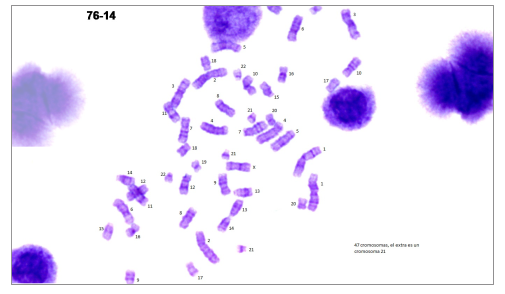
\includegraphics[width=0.8\textwidth]{Figs/Karyogram1}
     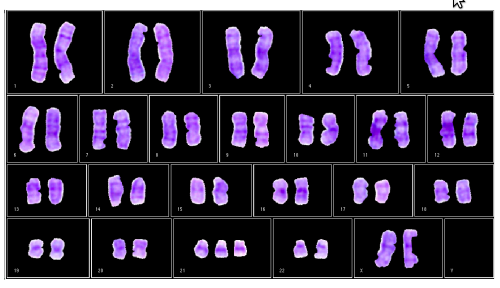
\includegraphics[width=0.8\textwidth]{Figs/Karyogram2}
     \end{center}
\end{column}
\end{columns}
\end{block} 
\footnotetext[1]{\fullcite{MarcoNuno_Revista_2020_04_00}}
\setcounter{footnote}{0}
\end{frame}


\begin{frame}{\citetitle{MarcoNuno_Revista_2020_04_00}  (2)}
\begin{block}{Proposed System} 


\begin{columns}
\begin{column}{0.6\textwidth}
Tasks performed by the proposed system:
		\begin{enumerate}
		\item Chromosome segmentation. 
\note[item]{... requires geometry analysis and image processing techniques related to pixel labelling.		}
        \item Feature extraction.
\note[item]{These features are: the 32 intensity values along medial axis, Perimeter, Area, Medial axis length, Intensity levels along 64 traversal lines touching the medial axis and Length of 64 traversal lines touching the medial axis. }		
\begin{center}
     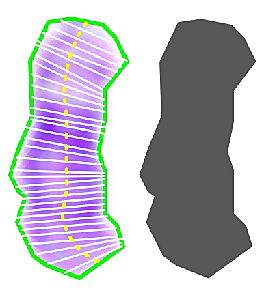
\includegraphics[width=0.25\textwidth]{Figs/Cromosomita2}
\end{center}

		\item Coarse and Fine Chromosome classification
\note[item]{    ... this classification is based on two main stages: a coarse classification where each chromosome is classified in one of three main groups; and a fine classification, where each chromosome in the coarse classification is assigned to one of the 24 chromosome types}		
%		\item Dedicated classification based on $G_1$, $G_2$ and $G_3$.
		%\item Merge chromosomes into karyogram.
		\item Finally, the chromosome classifications of each group are used to build tthe karyogram.  
		\end{enumerate}


\end{column}
\begin{column}{0.4\textwidth}  
    \begin{center}
     %%%%% this is a minipage, so \textwidth is already adjusted to the size of the column
     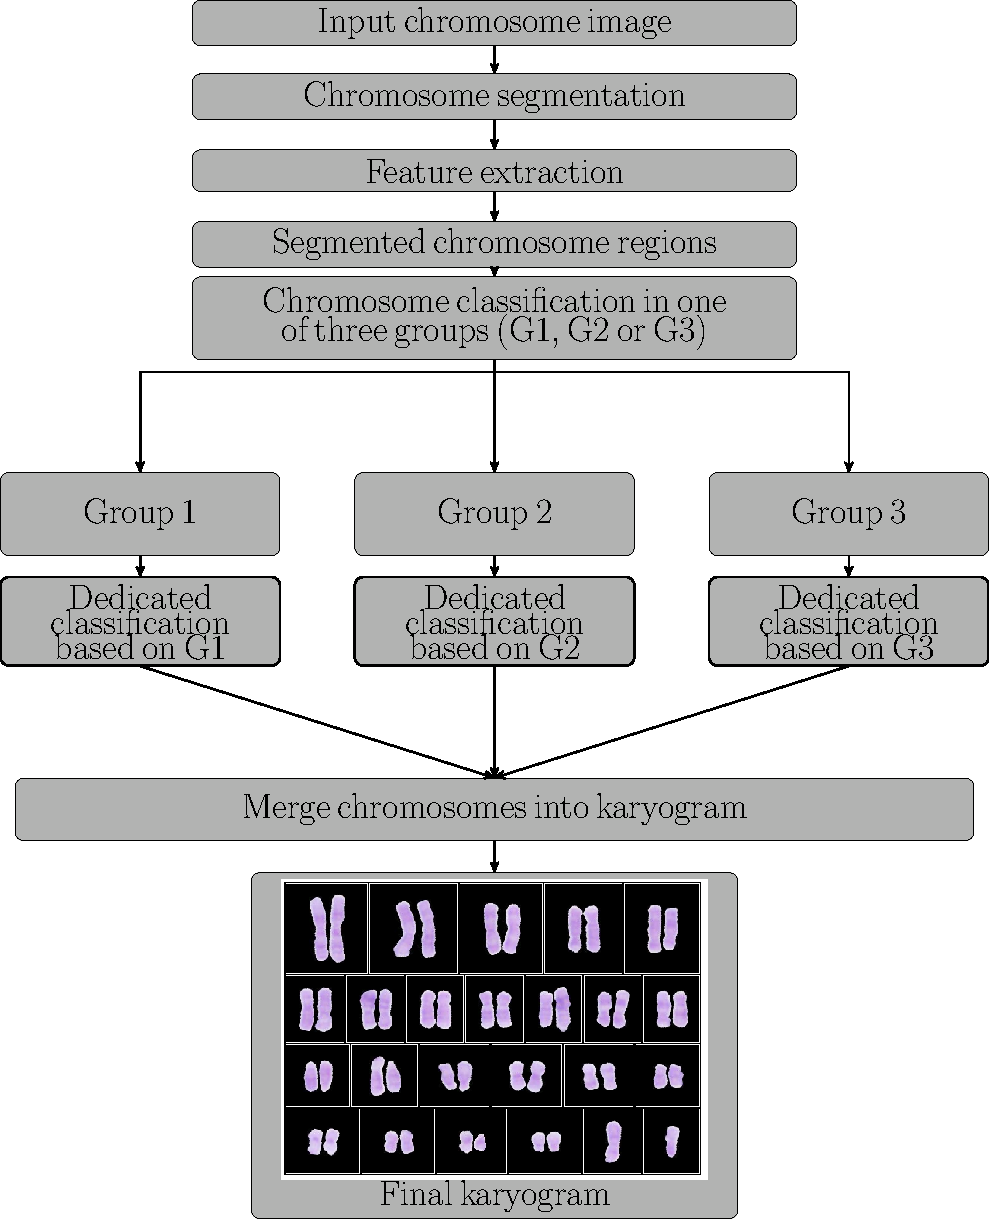
\includegraphics[width=0.75\textwidth]{Figs/Karyogram5}
     \end{center}
\end{column}
\end{columns}
\end{block} 
\end{frame}

\begin{frame}{\citetitle{MarcoNuno_Revista_2020_04_00}  (3)}
\begin{block}{Datasets, Tools and Results} 
\begin{columns}
\begin{column}{0.58\textwidth}
Datasets:
\begin{itemize}
\item 24 images provided by the Children’s Hospital of Tamaulipas (CHT).
\item 119 images from University of Padova.
\end{itemize}



Tools:
\begin{itemize}
\item Matlab was used for the image procesing.
% Preprocessing, segmentation and transformation required in order to separate the chromosomes from the input prometaphase image.
\item Weka 3.6.7 was used to train and test classifiers.
\end{itemize}

\note[item]{51 classifier algorithms were evaluated, and after several tests, a Multilayer Perceptron was detected as the classifier with the higher accuracy.  }
\note[item]{We based mainly on Neural Networks, and performed several experiments varying the number of neurons in the hidden layer} 
\note[item]{We used two types of NN architectures: multi-class and binary}
%\note[item]{In a Multi-class NN architecture, features are used to decide if the current chromosome belongs to one of the three groups.}
%\note[item]{In a Binary NN architecture, features are used to decide if a chromosome belongs or not to one of the three groups.}
\note[item]{We concluded that for this problem, using the few neurons in hidden layer we obtained the high accuracy in both NN architectures.}



\end{column}
\begin{column}{0.4\textwidth}



    \begin{center}
     %%%%% this is a minipage, so \textwidth is already adjusted to the size of the column
     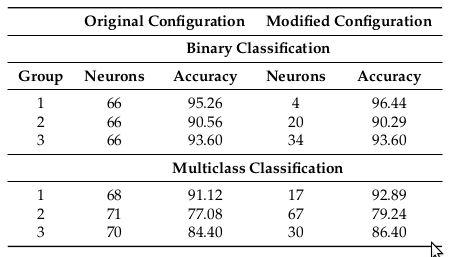
\includegraphics[width=0.96\textwidth]{Figs/Karyogram4}
     \end{center}
\end{column}
\end{columns}

\end{block} 
\end{frame}


